\chapter{Resultados}

O processo de seleção dos estudos, apresentado na Figura \ref{fig:dist}, consistiu em quatro etapas principais. Dos 860 resultados de pesquisa, 783 eram únicos (passo 2, Figura \ref{fig:dist}). Posteriormente, lendo o título e o resumo dos artigos, foram excluídos 673 estudos, baseados nos critérios de exclusão (passo 3). Quando não havia dados suficientes para exclusão, o trabalho foi deixado para o próximo passo. Depois de terminar o passo 3, 110 trabalhos permaneceram no processo de seleção. Depois de ler e analisar os 110 artigos deixados para a leitura de texto completo (passo 4), obtivemos 94 artigos relevantes. 

\begin{figure}[h!] %use h para forçar que a figura fique abaixo do texto
	\caption{Distribuição dos trabalhos na revisão.}
	\begin{center}
	    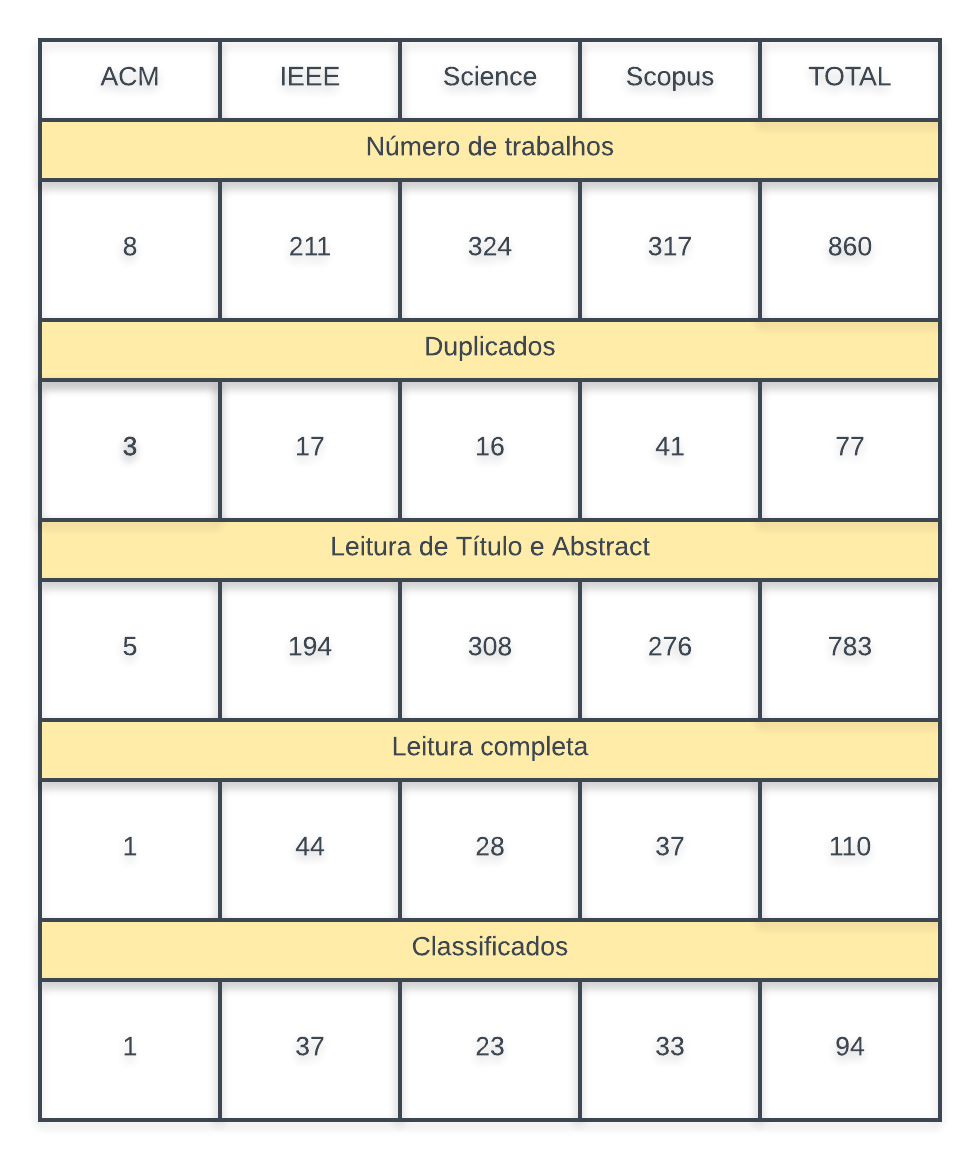
\includegraphics[scale=0.3]{figuras/revvisao.png} % altere o atributo scale para o tamanho da figura
	\end{center}
	\label{fig:dist}
	\legend{Fonte: Elaborado pelo autor.}
\end{figure}

\begin{comment}

\section{Avaliação de Qualidade}
   descritos na tabela \ref{tab:quality} cada critério podendo responder a três opções "Sim", "Não", "Parcialmente" sobre o dado relevante para a pesquisa, opções essas que impactam na pontuação geral do trabalho em respectiva ordem 1.0, 0.0, 0.5 cada trabalho podendo atingir um máximo de 12 e o mínimo em 5.0. Felizmente, nenhum trabalho foi excluído do estudo pela pontuação na avaliação de qualidade.
\end{comment} 


Os dados foram extraídos dos 94 estudos que satisfizeram os critérios de inclusão seguindo o formulário de extração descrito na Tabela \ref{tab:extraction}. Antes de apresentar os resultados e análises das perguntas de pesquisa, é fornecido uma visão geral das características gerais dos estudos.
\section{Visão geral dos estudos}

As bases de dados retornaram um total de 860 trabalhos sendo distribuídos em ACM: 8, IEEE: 211, Science: 324, Scopus: 317, a
disposição dos mesmos está ilustrada na Figura \ref{fig:grafartigosbase}.


\begin{figure}[h!] 
   	    \captionsetup{width=16cm}%Da mesma largura que a figura
		\Caption{\label{fig:grafartigosbase} Artigos por base.}
		\UFCfig{}{
			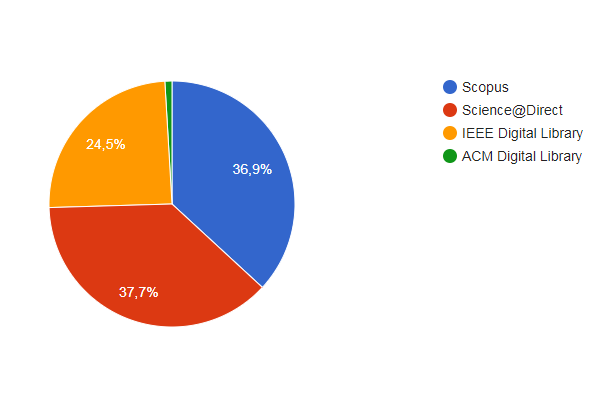
\includegraphics[width=13cm]{figuras/artigosbase}
		}{
			\Fonte{Ferramenta Parsif.al.}
		}	
	\end{figure}
Os trabalhos aceitos por cada base totalizaram 94 sendo distribuídos: ACM: 1, IEEE: 37, Science: 23, Scopus: 33, ver Figura \ref{fig:grafartigosacc}.


\begin{figure}[h!] 
   	    \captionsetup{width=16cm}%Da mesma largura que a figura
		\Caption{\label{fig:grafartigosacc} Artigos aceitos por base.}
		\UFCfig{}{
			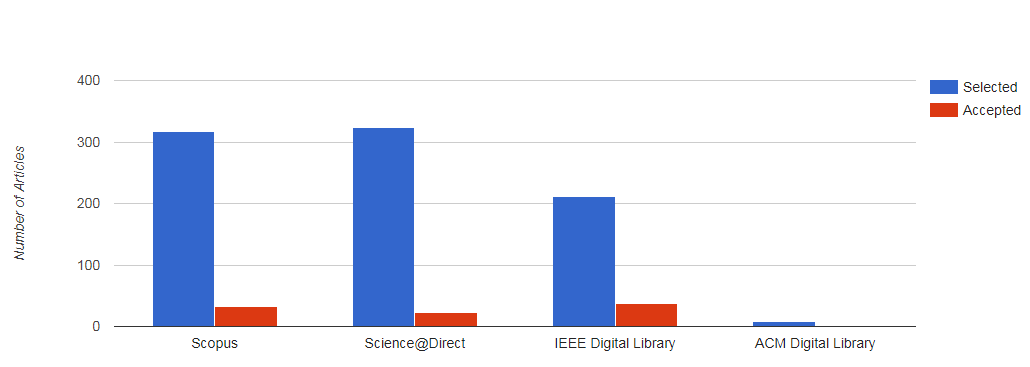
\includegraphics[width=13cm]{figuras/artigosbase1}
		}{
			\Fonte{Ferramenta Parsif.al.}
		}	
	\end{figure}



Constatou-se a importância da comunicação no âmbito da indústria e na academia, e o quão é notável que a pesquisa na comunicação no desenvolvimento de software é algo recorrente que cresceu ao longo dos anos como indica a figura que representa os anos de publicação dos trabalhos avaliados no estudo (ver Figura \ref{fig:camadas}).



\begin{figure}[h!] 
   	    \captionsetup{width=16cm}%Da mesma largura que a figura
		\Caption{\label{fig:camadas} Ano de publicação dos trabalhos.}
		\UFCfig{}{
			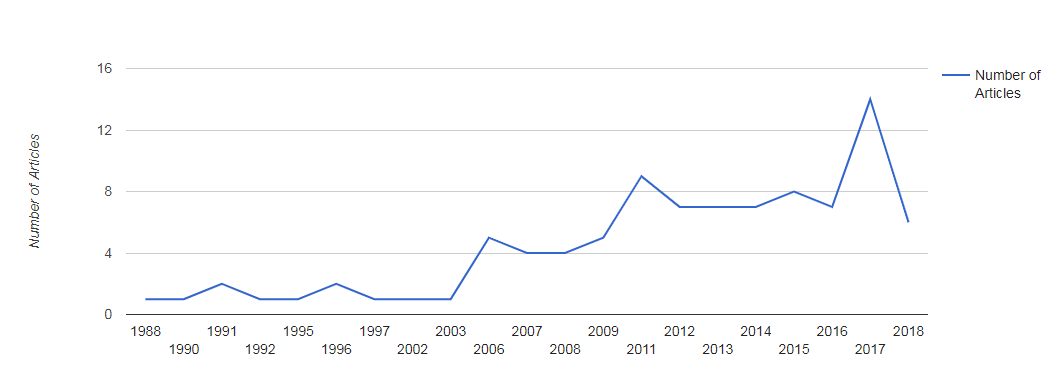
\includegraphics[width=16cm]{figuras/artigosbase2}
		}{
			\Fonte{Ferramenta Parsif.al.}
		}	
	\end{figure}


A extração dos dados mostrou que a pesquisa na área de comunicação de requisitos é relevante, a tabela a seguir contém autores de pelo menos três artigos avaliados neste estudo.

\begin{table}[h!]
\label{tab:autores1}
\caption{Autores com três ou mais trabalhos avaliados neste estudo.}
\begin{tabular}{|p{5cm}|p{9cm}|}
\hline
\textbf{Autores}                                     &                  \textbf{Referências}                                                                                                               \\ \hline
Kai Stapel                                          &

\cite{Stapel} 
\cite{stapel2011flow}
\cite{knauss2013v}
\cite{knauss2014openness}
\cite{knauss2012detecting}
                \\ \hline
Eric Knauss                                         &
\cite{knauss2013v}
\cite{knauss2014openness}
\cite{knauss2012detecting}
                \\ \hline
Daniela Damian                                     &         
\cite{6606709}
\cite{knauss2014openness}
\cite{damian2008need}
\cite{knauss2012detecting}

                                                                          \\ \hline
Elizabeth Bjarnason                                 &
\cite{bjarnason2017role}
\cite{bjarnason2012evidence}
\cite{bjarnason2011requirements}

                                                                           \\ \hline
Yu-Cheng Tu                                           &

\cite{tu2016experiment}
\cite{6130643}


                         \\ \hline
\end{tabular}
\Fonte{Elaborado pelo autor}
\end{table}


Nas próximas seções, são apresentadas as respostas para as perguntas da revisão sistemática.



\begin{comment}
Stakeholders envolvidos P1
Metodologia de desenvolvimento de
software
Ágil, tradicional, evolucionária, etc. P2
Domínio da empresa P3
Problemas de comunicação P4
Fator de comunicação P5
Impacto do fator de comunicação P6
Aspecto do processo de comunicação
afetado
P7
Canal de comunicação utilizado P8
Ferramentas utilizadas P8
Desafios em aberto
\end{comment}

\section{P1. Quais são os stakeholders envolvidos?}

A Figura \ref{fig:grafpap} ilustra a quantidade dos papéis desempenhados pelos stakeholders envolvidos no processo de desenvolvimento presentes nos estudos selecionados. Observou-se uma frequência maior de ``Clientes'', ``Desenvolvedores'' e ``Engenheiro de requisitos''. %, sendo assim determinante uma maior ocorrência de fatores durante a fase de elicitação de requisitos.

\begin{figure}[h!] %use h para forçar que a figura fique abaixo do texto
	\caption{Stakeholders citados nos estudos selecionados.}
	\begin{center}
	    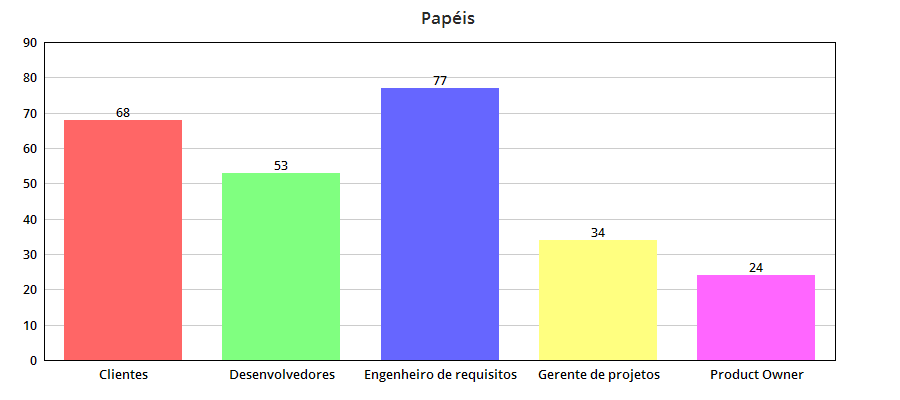
\includegraphics[scale=0.4]{figuras/grafpap.png} % altere o atributo scale para o tamanho da figura
	\end{center}
	\label{fig:grafpap}
	\legend{Fonte: Elaborado pelo autor.}
\end{figure}

\section{P2. Quais são os problemas de comunicação reportados no estudo?}

Observou-se que o maior deficit de comunicação está relacionado na fase de elicitação, já espera-se que seja uma fase crítica pois lida com a fase de indivíduos de domínios diferentes que necessitam trocar informações.
A natureza dos problemas em maior parte mostrou-se de origem humana e organizacional, podendo concluir então que uma abordagem nessas áreas poderia vir a melhorar o fluxo de comunicação.

\section{P3. Quais são os fatores de comunicação apontados no estudo?}

A partir da análise dos trabalhos selecionados foi identificado um total de 38 fatores distribuídos em 22 positivos e 16 negativos que afetam direta ou indiretamente na comunicação de requisitos no desenvolvimento de software,  Identificou-se que os fatores possuem naturezas diversas sendo bem evidentes a natureza sociocultural e organizacional, além disso a maioria dos fatores afeta em mais de um aspecto do processo de comunicação.

Os estudos selecionados evidenciaram que projetos com equipes dispersas globalmente sofrem problemas severos na comunicação. Observou-se também que o entendimento do domínio na elicitação de requisitos entre as partes envolvidas auxilia na comunicação assim como técnicas de elicitação já conhecidas. Outro fator preponderante na comunicação é a confiança entre o emissor e receptor, assim como fatores como requisitos vagos e incompletos.

Distâncias cognitivas, o tipo de linguagem, idiomas e metodologias ágeis também obtiveram uma representação considerável na pesquisa. Também é importante ressaltar que a inexistência de alguns dos fatores positivos pode acarretar em um problema na comunicação ou um pior processo no repasse de informações. Os fatores que influenciam positivamente na comunicação estão descritos na Tabela \ref{tab:fatoresP}.

%\usepackage{longtable}
\begin{longtable}{|p{5cm}|p{10cm}|}
\caption{Lista de Fatores Negativos.}

%\begin{longtable}[]
%\begin{tabular}{|p{6cm}|p{9cm}|}
\hline
\textbf{Fatores Positivos}                                                    & \textbf{Referência}                                                \\ \hline
Conhecimento do domínio                                                       & \cite{herbsleb2007global} \cite{hilbrich2017enforcing} \cite{schneider2017reframing} \cite{gates1997identification} \cite{aranda2009analyzing}  \cite{5457325},                                       \\ \hline
Uso de Vídeos/Videoconferência                                                & \cite{Oran:2017:ARC:3131151.3131166}, \cite{calazans2017software}  \cite{alnuem2012requirements} \cite{ali2016method} \cite{korkala2009distributed}
            \\ \hline
Metodologia ágil em ambientes globais                                         & \cite{knauss2014openness} \cite{noordeloos2012rup} \cite{wilks2012self} \cite{wongthongtham2006ontology} \cite{Hess2018}             \\ \hline
Documentação técnica e precisa                                                & \cite{soltani2015cross}\cite{knauss2014openness}, \cite{liskin2015artifacts} \cite{PERNSTAL201544} 
    \\ \hline
Comunicação cara a cara                                                       & \cite{wongthongtham2006ontology} \cite{Hess2018} \cite{aranda2009analyzing}
 \cite{korkala2009distributed}                                           \\ \hline
Uso de UML                                                                    & \cite{wasson2006case} \cite{diel2016communication} \cite{schneider2017reframing}, \cite{karlsson2007requirements}                   \\ \hline
Uso da linguagem nativa entre comunicadores                                   & \cite{aranda2009analyzing} \cite{6337317}             \cite{Takura19961716}                                                            \\ \hline
Interação constante                                                           & \cite{noordeloos2012rup} \cite{marnewick2011perspective} \cite{dos2013impact}  
            \\ \hline
Especificação de requisitos precisa                                          & \cite{5457325} \cite{tu2016experiment} \cite{unknown2006}
 \cite{Takura19961716}            
        \\ \hline
Comunicação entre os usuários e o engenheiro de requisitos                    &  \cite{hagelstein1988declarative} \cite{laporti2009athena}             \cite{8051365}                                                       \\     \\\hline
Contato próximo com os usuários                                               & \cite{hagelstein1988declarative} \cite{laporti2009athena}             \cite{Rauterberg1995391}                                              \\     \\\hline
Uso de sistemas de controle de versão                                         &    \cite{wasson2006case} \cite{6606709}                                \\ \hline
Analista de requisitos com proficiência em comunicação                        & \cite{sedelmaier2017can} \cite{Anwar2016726}                '            \\ \hline
Fóruns de discussão                                                           & \cite{alnuem2012requirements} \cite{8051365}                          \\ \hline
Maior transparência em documentos                                             & \cite{Oran:2017:ARC:3131151.3131166}     \cite{liskin2015artifacts}                                                     \\ \hline
Uso de Mockup e protótipos                                                    & \cite{Oran:2017:ARC:3131151.3131166} \cite{calazans2017software}        
            \\ \hline

Ferramenta de comunicação em grupos                                           &  \cite{bjarnason2017role}                                                \\ \hline
Prontidão de resposta                                                         & \cite{KIRITANI2015153}                                                    \\ \hline


Abordagem organizacional que permita fluxo aberto de mensagens                & \cite{6051643}                                                         \\ \hline





Uso de histórias do usuário                                                   & \cite{knauss2012detecting}                                            \\ \hline


Discussões contextuais em torno dos requisitos                                & \cite{stapel2009using}                                                  \\ \hline

Comunicação humana escrita com figuras, diagramas ou tabelas para sua clareza & \cite{8267930}                                                           \\ \hline


\caption{Fonte: Elaborado pelo autor}
%\end{tabular}
\label{tab:fatoresP}


\end{longtable}
\newpage

%\legend {\fontsize{10}{12}\selectfont {Fonte: Elaborado pela autor.}}
Os fatores que influenciam negativamente a comunicação estão descritos na Tabela \ref{tab:fatoresN}. 

\begin{longtable}{|p{5cm}|p{10cm}|}
%\begin{tabular}{|p{6cm}|p{9cm}|}
\caption{Fatores Negativos}

\hline
\textbf{Fatores Negativos}                                   & \textbf{Referência}                                                                                                                                                                                                                                                                                                                                                       \\ \hline

Diferenças socioculturais                                    & %\begin{tabular}[c]{@{}l@{}} 
\cite{herbsleb2007global}
\cite{wasson2006case}
\cite{diel2016communication}
\cite{alnuem2012requirements}
\cite{noordeloos2012rup}
\cite{aceituna2014model}
\cite{khan2014proposed}
\cite{Mohamad2017179}
\cite{Ghanbari201532}
\cite{5457325}\cite{aranda2009analyzing}\cite{6743519}\cite{6337317}\cite{8357767}\cite{unknown}\cite{korkala2009distributed}
%\end{tabular}                                              
\\ \hline
Distância geográfica                                         & 
\cite{wasson2006case}\cite{diel2016communication}\cite{alnuem2012requirements}\cite{noordeloos2012rup}\cite{mellhorn2017improving}\cite{calazans2017software}\cite{liskin2012improving}\cite{wongthongtham2006ontology}\cite{aceituna2014model}\cite{khan2014proposed}\cite{jeffrey1996addressing}\cite{5457325}\cite{6743519}\cite{6337317}\cite{8357767} \cite{Bjarnason2017}\cite{korkala2009distributed}

\\ \hline
Falta de confiança entre a equipe                            & 
\cite{diel2016communication}
\cite{noordeloos2012rup}\cite{xia2017personality}\cite{wu2015analysis}\cite{marnewick2011perspective}\cite{kiritani2015success}\cite{khan2014proposed}\cite{unknown}\cite{unknown2006}\cite{Anwar2016726}
            
\\ \hline
Requisitos vagos e incompletos                               & 
\cite{soltani2015cross} \cite{karlsson2007requirements}\cite{kiritani2015success}\cite{ali2016method}\cite{Jarke2011992} \cite{Ghanbari201532}                                       \\ \hline
Exclusão e distorção de informações                          &  \cite{echeverria2017influence}\cite{soltani2015cross}\cite{cois2014modern}\cite{sinha2006enabling}\cite{aceituna2014model}\cite{Tu2016}                                                                                       \\ \hline
Falta de compreensão mútua                                   &  \cite{wu2015analysis}\cite{karlsson2007requirements}\cite{khan2014proposed}\cite{unknown}\cite{Amrit:2017:EME:3084381.3084413}                                                                                                                                             \\ \hline
Diferentes idiomas falados por partes interessadas      &      \cite{pilat2011knowledge} \cite{mahmood2013software} \cite{khan2014proposed}                                                                                                                                                                                                         \\ \hline
Distâncias cognitivas (diferenças de conhecimento)           &                      \cite{mellhorn2017improving}  \cite{pilat2011knowledge}  \cite{maier2006identifying}                                                                                                                                                                                                                 \\ \hline
Frequência de comunicação baixa                              &                          \cite{diel2016communication}           \cite{marnewick2011perspective}                                                             \\ \hline
Limitação técnica no projeto                                 &       \cite{bjarnason2017role} \cite{sedelmaier2017can}                            \\ \hline
Incertezas do cliente quanto aos requisitos                  &  \cite{soltani2015cross}
\\ \hline

Incluir mais requisitos do que o especificado                &            \cite{bjarnason2011requirements}
\\ \hline


Participação inadequada dos clientes                         &             \cite{Ghanbari201532}
\\ \hline
Ambiguidade em escrita de história de usuário e casos de uso &                                                                                                                                          \cite{mahmood2013software}                                                                                                                                                                                                              \\ \hline
Falta de entendimento do canal de comunicação                &                                                                                                                                                                                                              \cite{mellhorn2017improving}                                                                                                                                        \\ \hline

\caption{Fonte: Elaborado pelo autor}

%\end{tabular}
\label{tab:fatoresN}

\end{longtable}

\newpage

 A Figura \ref{fig:graf2} ilustra a  ocorrência dos fatores positivos que apareceram quatro vezes ou mais nos estudos selecionados.



	\begin{figure}[h!] 
   	    \captionsetup{width=16cm}%Da mesma largura que a figura
		\Caption{\label{fig:graf2} Ocorrência dos fatores positivos.}
		\UFCfig{}{
			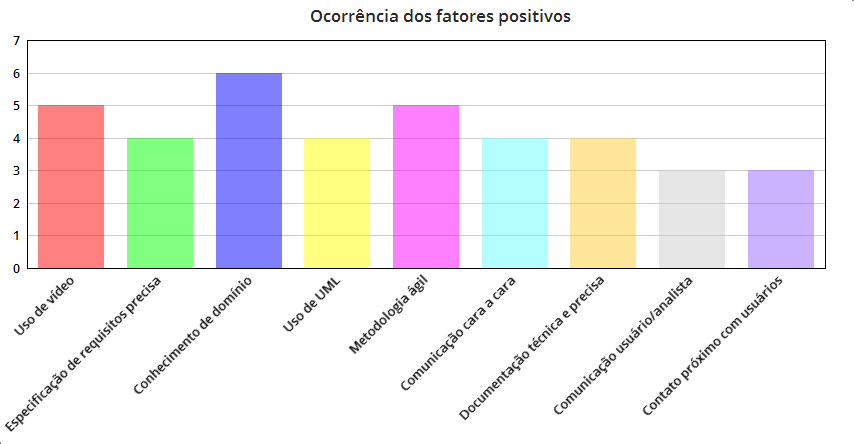
\includegraphics[width=16cm]{figuras/ChartGo.png}
		}{
			\Fonte{Fonte: Elaborado pelo autor.}
		}	
	\end{figure}
   
Na ocorrência de fatores negativos observou-se que fatores de natureza humana sobressaíram em relação aos outros. A Figura \ref{fig:ocnega}
ilustra a ocorrência de fatores negativos que surgiram quatro vezes ou mais na pesquisa. 
   

\begin{figure}[h!] 
   	    \captionsetup{width=16cm}%Da mesma largura que a figura
		\Caption{\label{fig:ocnega} Ocorrência dos fatores negativos.}
		\UFCfig{}{
			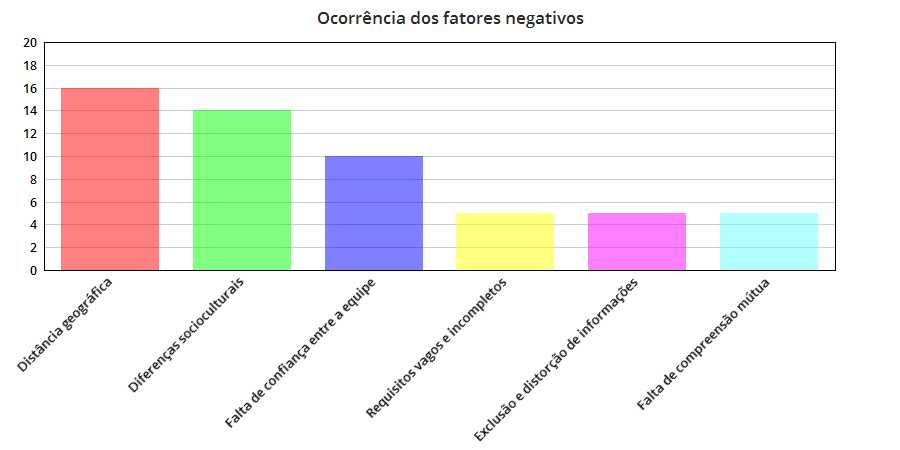
\includegraphics[width=16cm]{figuras/ocnega.png}
		}{
			\Fonte{Fonte: Elaborado pelo autor.}
		}	
	\end{figure}
   

\section{P4. Qual o impacto do fator de comunicação?}

 Foi realizado um levantamento do impacto dos fatores no processo de engenharia de requisitos considerando a escala ``grave'', ``médio'' e ``leve'', Sendo considerado grave todo e qualquer fator que acarretasse na oclusão e distorção de informações e ocorressem com maior frequência, médio fatores que causassem falhas na comunicação com uma frequência branda, e leve fatores que causassem apenas simples falhas.
 
 
 Os resultados ajudam a validar o quão a comunicação é importante na etapa de engenharia de requisitos. Por consenso foi acordado que todos os fatores afetam entre ``grave'' e ``médio'' em requisitos, visto que todos têm a possibilidade de causar distorções e falta de informações relevantes no fluxo de requisitos.
 
    Sendo descritos como graves os seguintes fatores: 
"Diferenças socioculturais", "Falta de colaboração de desenvolvedores", "Falta de confiança entre a equipe", "Distância geográfica", "Frequência de comunicação baixa", "Incertezas do cliente quanto aos requisitos" e "Requisitos Vagos e incompletos" o restante sendo classificado como de médio impacto, os resultados estão ilustrados na Figura \ref{fig:grafimpact}.


\begin{figure}[h!] %use h para forçar que a figura fique abaixo do texto
	\caption{Percentual do impacto dos fatores.}
	\begin{center}
	    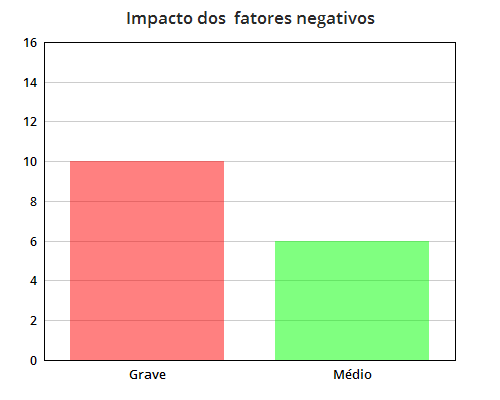
\includegraphics[scale=0.5]{figuras/impact.png} % altere o atributo scale para o tamanho da figura
	\end{center}
	\label{fig:grafimpact}
	\legend{Fonte: Elaborado pelo autor.}
\end{figure}

\section{P5. O fator interfere em qual aspecto do processo de comunicação?}

Os resultados demonstram uma maior ocorrência de fatores positivos afetando o canal de comunicação como demonstrado na Figura \ref{fig:graf}. Sendo assim, é possível inferir que os canais de comunicação bem definidos e eficientes são de grande relevância na engenharia de requisitos. 

\newpage
   \begin{figure}[h!] %use h para forçar que a figura fique abaixo do texto
    \caption{Fatores positivos no processo de comunicação.}
	\begin{center}
	    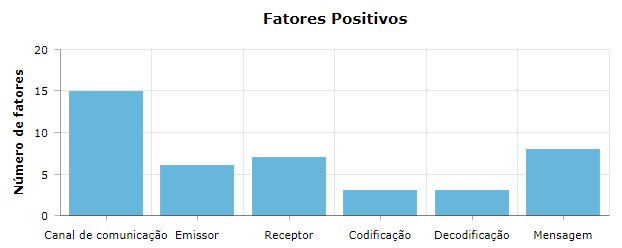
\includegraphics[scale=0.9]{figuras/graftcc} % altere o atributo scale para o tamanho da figura
	\end{center}
	\label{fig:graf}
	\legend{Fonte: Elaborado pelo autor.}
\end{figure}

Os fatores negativos ocorrem com maior frequência na emissão e recepção de dados na comunicação, com destaque também para a codificação e decodificação visto que estão estreitamente correlacionados. Este fato evidencia que o problema ocorre em repassar e receber dados e requisitos de forma correta.  

\begin{figure}[h!] %use h para forçar que a figura fique abaixo do texto

	\begin{center}
	    \caption{Fatores negativos no processo de comunicação.}
	    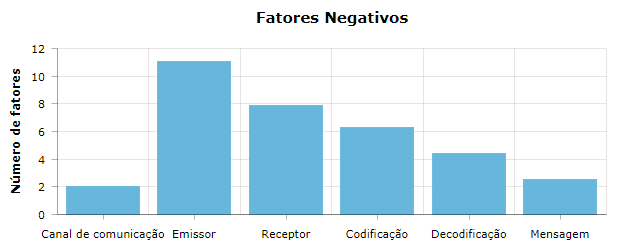
\includegraphics[scale=0.9]{figuras/graftcc1} % altere o atributo scale para o tamanho da figura
	\end{center}
	\label{fig:graft}
	\legend{Fonte: Elaborado pelo autor.}
\end{figure}

   
\section{Modelo de classificação dos fatores}

A construção do modelo foi realizada observando em qual aspecto o fator afeta no processo de comunicação, possibilitando assim obter uma classificação dos fatores regida pelo processo de comunicação, dessa forma obtém-se uma visão geral disposta em quadros que identificam os fatores positivos e negativos, podendo obter informações de quais fatores são, onde atuam e se seu impacto é benéfico ou prejudicial. 

\subsection{Fatores no canal de comunicação}

Foi identificado que os estudos levantados nessa pesquisa relatam que o canal de comunicação bem definido e técnico possui capacidade efetiva de repassar informações, Observou-se também que técnicas de elicitação atuando como canal de comunicação se tornam bastante eficazes no que propõem (ver Figura \ref{fig:quadro1}).
 
\begin{figure}[h!] %use h para forçar que a figura fique abaixo do texto
    \caption{Canal de comunicação - Fatores positivos.}
	\begin{center}
	    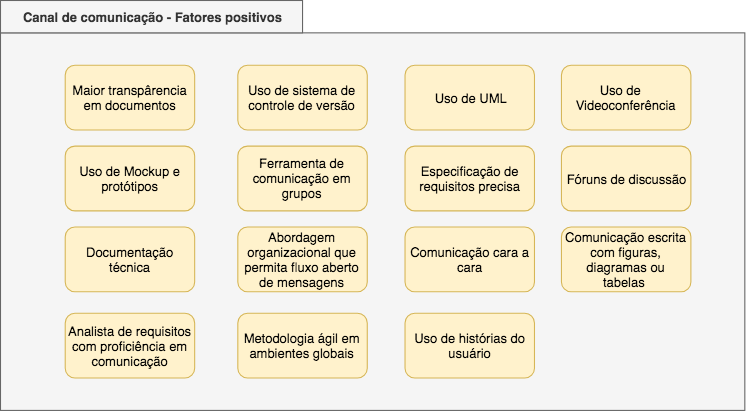
\includegraphics[scale=0.6]{figuras/quadro1} % altere o atributo scale para o tamanho da figura
	\end{center}
	\label{fig:quadro1}
	\legend{Fonte: Elaborado pelo autor.}
\end{figure}


Em contrapartida somente dois fatores negativos são relacionados ao canal de comunicação como ilustrado na Figura \ref{fig:quadro2}.
\newpage
\begin{figure}[h!] %use h para forçar que a figura fique abaixo do texto
\caption{Canal de comunicação - Fatores negativos.}
	\begin{center}
	    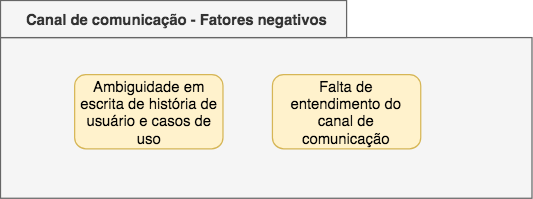
\includegraphics[scale=0.6]{figuras/quadro2} % altere o atributo scale para o tamanho da figura
	\end{center}
	\label{fig:quadro2}
	\legend{Fonte: Elaborado pelo autor}
\end{figure}

\subsection{Fatores de comunicação em emissor e receptor}

Os fatores positivos relacionados ao emissor e receptor são estritamente correlacionados, pois a emissão e recepção de uma mensagem é assíncrona, ou seja, o receptor ora pode se comportar como emissor e vice e versa, com exceção do fator "Prontidão de resposta" que diz respeito somente ao receptor (ver Figura \ref{fig:quadro3} e \ref{fig:quadroneg}).


\begin{figure}[h!] %use h para forçar que a figura fique abaixo do texto
\caption{Emissor - Fatores positivos.}
	\begin{center}
	    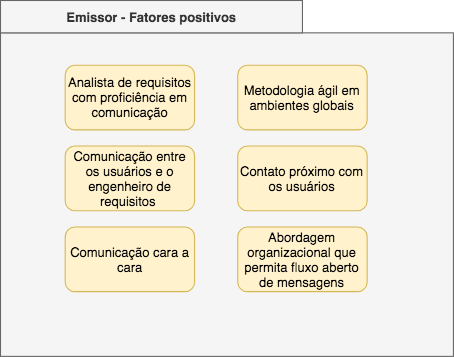
\includegraphics[scale=0.6]{figuras/quadro3} % altere o atributo scale para o tamanho da figura
	\end{center}
	\label{fig:quadro3}
	\legend{Fonte: Elaborado pelo autor.}
\end{figure}

\newpage


\begin{figure}[h!] %use h para forçar que a figura fique abaixo do texto
	\begin{center}
	
	\caption{Receptor - Fatores positivos.}
		\label{fig:quadroneg}
	    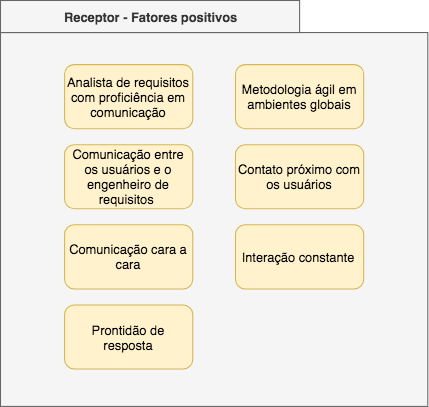
\includegraphics[scale=0.6]{figuras/quadro4} % altere o atributo scale para o tamanho da figura
	\end{center}

	\legend{Fonte: Elaborado pelo autor.}
\end{figure}

Nos fatores negativos no emissor e receptor existe uma recorrência de influência em falhas e ruídos de comunicação nesses aspectos, o que evidencia que no desenvolvimento de software é importante uma abordagem que melhore a relação emissor/receptor que ocorre em todo o processo de desenvolvimento (ver Figura \ref{fig:quadro5} e \ref{fig:quadro6}).

\begin{figure}[h!] %use h para forçar que a figura fique abaixo do texto
	\begin{center}
	    \caption{Emissor - Fatores negativos.}
	    \label{fig:quadro5}
	    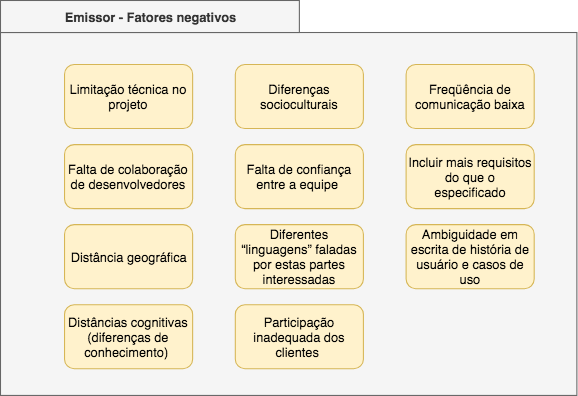
\includegraphics[scale=0.55]{figuras/quadro5} % altere o atributo scale para o tamanho da figura
	\end{center}
	
	\legend{Fonte: Elaborado pelo autor}
\end{figure}
\begin{figure}[h!] %use h para forçar que a figura fique abaixo do texto

	\begin{center}
	    \caption{Receptor - Fatores negativos.}
	    	\label{fig:quadro6}
	    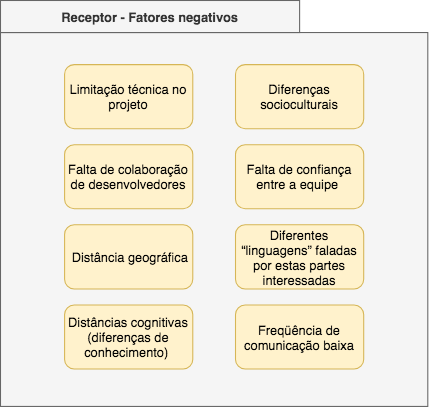
\includegraphics[scale=0.55]{figuras/quadro6} % altere o atributo scale para o tamanho da figura
	\end{center}

	\legend{Fonte: Elaborado pelo autor.}
\end{figure}

\subsection{Fatores de comunicação em codificação e decodificação}
Os fatores em codificação e decodificação assim como emissor e receptor são altamente atrelados visto que uma mensagem exige o mesmo conhecimento por parte do emissor para codifica-lá e tal qual o receptor para decodifica-lá, os mesmos se mostraram peculiares e restritos, e exclusivamente de natureza técnica organizacional e sociocultural (Ver Figura \ref{fig:quadro7}).

\begin{figure}[h!] %use h para forçar que a figura fique abaixo do texto
	\begin{center}
	    \caption{Codificação e decodificação - Fatores Positivos.}
	    \label{fig:quadro7}
	    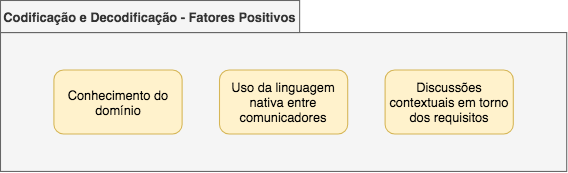
\includegraphics[scale=0.6]{figuras/quadro7} % altere o atributo scale para o tamanho da figura
	\end{center}
	
	\legend{Fonte: Elaborado pelo autor.}
\end{figure}

Para reforçar, os fatores negativos nos mesmos atuam em falhas humanas de comunicação, ex: "falta de compreensão mútua", "incerteza do cliente quanto aos requisitos" assim como falhas organizacionais (Ver Figura \ref{fig:quadro8}). 


\begin{figure}[h!] %use h para forçar que a figura fique abaixo do texto
	\begin{center}
	    \caption{Codificação e decodificação - Fatores negativos.}
	    	\label{fig:quadro8}
	    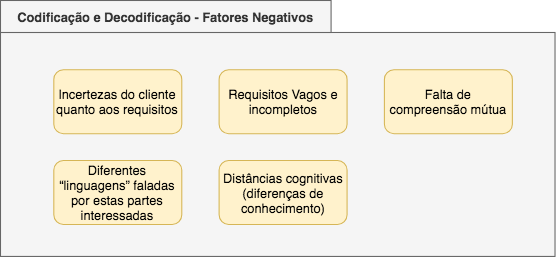
\includegraphics[scale=0.6]{figuras/quadro8} % altere o atributo scale para o tamanho da figura
	\end{center}

	\legend{Fonte: Elaborado pelo autor.}
\end{figure}

\subsection{Fatores de comunicação em mensagens}

A mensagem é relacionada com o canal de comunicação, visto que é a partir do canal que a mensagem flui, os fatores positivos em mensagem foram justamente a aplicação dos canais de comunicação já eficientes na elicitação de requisitos (Ver Figura \ref{fig:quadro9}), destacando os fatores "Maior transparência em documentos" e  "Documentação técnica" que definem uma abrangência considerável na engenharia de requisitos.


\begin{figure}[h!] %use h para forçar que a figura fique abaixo do texto
	\begin{center}
	    \caption{Mensagem - Fatores positivos.}
	    	\label{fig:quadro9}
	    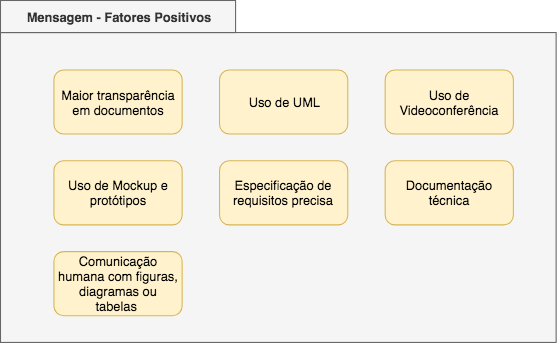
\includegraphics[scale=0.6]{figuras/quadro9} % altere o atributo scale para o tamanho da figura
	\end{center}

	\legend{Fonte: Elaborado pelo autor.}
\end{figure}

O impacto dos fatores negativos em mensagem se mostraram altamente prejudiciais, levando em conta que os mesmos dizem respeito a distorcer, excluir e diminuir a informação que deve ser repassada, algo que pode acarretar falhas graves se tratando de requisitos (ver Figura \ref{fig:quadro10}). 

\begin{figure}[h!] %use h para forçar que a figura fique abaixo do texto
	\begin{center}
	    \caption{Mensagem - Fatores negativos.}
	    	\label{fig:quadro10}
	    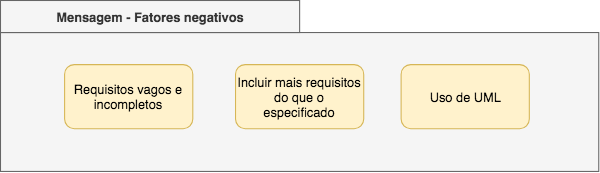
\includegraphics[scale=0.6]{figuras/quadro10} % altere o atributo scale para o tamanho da figura
	\end{center}

	\legend{Fonte: Elaborado pelo autor.}
\end{figure}

%{tabular}{|p{2.5cm}|p{2.2cm}|p{2.0cm}|p{2.0cm}|p{2.0cm}| }

A próxima seção apresenta a conclusão e propostas de trabalhos futuros. 

\newpage















   

